%%%%%%%%%%%%%%%%% TOMA DE REQUISITOS %%%%%%%%%%%%%%%%%%%%%%%5
\section{Toma de requisitos}

\paragraph{}
Para la creación de cualquier producto software, es necesario establecer las distintas condiciones y necesidades que
ha de satisfacer. Seguiremos un esquema que nos permita describir los requisitos de una forma metódica y racional.
%\paragraph{}

\subsection{Requisitos de interfaces externas}

\paragraph{}
En este apartado se describirá los requisitos de conexión del software y el hardware, así como la interfaz de usuario.

\paragraph{}
La conexión entres el software y el hardware se encarga la librería \emph{SDL}, mediante el wrapper \emph{Pygame} para 
el lenguaje de programación \emph{Python}. Por lo que al ser un sistema preestablecido, no será necesario realizar el diseño,
ni el análisis, sólo haremos uso de él.

\paragraph{}
Así que pasamos a definir la interfaz entre el usuario y el videojuego. Todas las ventanas de la aplicación tendrán una 
resolución de 800x600 píxeles, siendo posible establecer el modo de pantalla completa \footnote{El modo de pantalla completa
se podrá establecer a través del menú de opciones}. A continuación se distinguen las distintas
ventanas que el usuario encontrará en el sistema:

\begin{description}
    \item \textbf{Ventana de introducción} En esta primera ventana se mostrará únicamente el logotipo del juego, situando al usuario en
    contexto para introducirlo en la ejecución de la apliación.
    
    \item \textbf{Ventana de menú principal} La ventana del menú principal muestra el menú de inicio de \emph{Zycars}, asi como 
    todas las opciones generales del juego diponibles, que son las siguientes:
        \begin{itemize}
            \item Carrera Rápida
            \item Campeonato
            \item Contrarreloj
            \item Opciones
            \item Salir
        \end{itemize}
        En este menú y en los siguiente que se describan se usará el raton para navegar por ellos y solo será necesario
        un click sobre la opción deseada para acceder a ella.
    
    \item \textbf{Ventana de opciones} Desde la ventana de opciones se podrán modificar las distintas carácteristicas de la 
    configuración del juego como el audio o controles. Esta ventana se podría dividir en tres partes diferencias que se indican
    a continuación:
        \begin{itemize}
            \item Opciones de audio: podremos modificar el volumen de efectos de sonido y música del juego. También estará la opción
            de silenciar cualquier tipo de sonido.
            
            \item Opciones de pantalla: a través de esta ventana podremos activar o desactivar el modo de pantalla completa.
            
            \item Opciones de control: en esta ventana podremos modificar los controles del juego. Tanto de dirección, lanzamiento
            de items y pausa del juego.
        \end{itemize}
    
    \item \textbf{Ventana de selección de personaje} Esta ventana será compartida por los tres modos de juego disponibles. En ella 
    podremos elegir al personaje que desearemos controlar a lo largo de las carreras. De estos jugadores se nos mostrarán sus 
    distintas habilidades.
    
    \item \textbf{Ventana de selección de circuito} Ventana compartida por el modo carrera rápida y contrarreloj. En esta ventana
    deberemos elegir el circuito en el que deseamos competir. Se nos mostrará una imagen de cada circuito que seleccionemos.
    
    \item \textbf{Ventana de selección de campeonato} Ventana muy similar a la descrita anteriormente. En ella se nos mostrarán
    todos los circuitos de cada campeonato disponible. Pero al contrario que la anterior en esta ventana elegiremos el campeonato 
    del circuito seleccionado en el momento.
    
    \item \textbf{Ventana de juego} Ventana principal de todo el juego. Mostrará la carrera actual que se esté disputando, así como
    los distinto marcadores aclaratorios sobre el estado de la carrera, como pueden ser posiciones de los jugades, item actual y
    tiempos de carrera. Según la tecla índicada en los controles del menú de opciones (ESC o p) se podrá acceder al menú
    de pausa del juego.
    
    \item \textbf{Ventana de pausa} Únicamente accesible desde la ventana de juego. Esta nos permitirá detener el juego en curso, 
    siendo posible reaundar el juego, reiniciar el mismo o volver al menú principal.
    
    \item \textbf{Ventana de posiciones de carrera} Ventana mostrada al terminar alguna de las carreras. En ella nos muestra el 
    resultado de la última carrera disputada. Nos pertime continuar al siguiente circuito, en el caso del modo campeonato, o seguir
    hacia el menú principal, en el modo carrera rápida. También se nos permite reniciar la última carrera disputada.
    
    \item \textbf{Ventana de posiciones de campeonato} Ventana mostrada en el modo campeonato tras la ventana de posiciones 
    de carrera, en ella se nos muestra las posiciones de los competidores en el campeonato actual.
    
    \item \textbf{Ventana de tiempos de contrarreloj} Ventana mostrada al completar algún circuito en el modo contrarreloj. En ella
    se nos muestran los distintos tiempos conseguidos a lo largo del circuito y se nos indicará si hemos batido algún record.
    Esta ventana nos permite continuar hacia el menú principal, así como reiniciar el circuito disputado.
    
\end{description}

\subsection{Requisitos funcionales}

\paragraph{}
Los requisitos funcionales que el sistema debe ofrecer son los siguientes:

\begin{itemize}
    \item Salir de la aplicación desde cualquier ventana.
    \item Seleccionar los distintos modos de juego.
    \item Permitir al jugador competir contra la inteligencia artificial.
    \item Modificar la configuración (audio, pantalla y controles) del juego.
    \item Pausar el juego.
    \item Seleccionar uno de los jugadores propuestos.
    \item Seleccionar cualquiera de los circuitos disponibles.
    \item Seleccionar cualquiera de los campeonatos disponibles.
    \item Reiniciar cualquier carrera una vez terminada o en curso.
    \item Reiniciar cualquier campeonato una vez terminado o en curso.
    \item Lanzamientos de items durante cualquier carrera.
\end{itemize}

\paragraph{}
Los distintos tipos de jugadores son:

\begin{itemize}
    \item \textbf{Humano}: es el controlado por una persona
    \item \textbf{Inteligencia artificial}: controlado por el ordenador.
\end{itemize}

\paragraph{}
Existes tres modos de juego:

\begin{itemize}
	\item \textbf{Carrera rápida}: consiste en la realización de un único circuito, compitiendo contra la inteligencia artificial.
	\item \textbf{Campeonato}: el jugador competirá contra la inteligencia artificial a lo largo de 4 carreras, en las que obtendrá una puntuación
	según la posición obtenida en cada una de las carreras. El ganador será el que mejor puntuación haya conseguido al concluir
	el campeonato.
	\item \textbf{Contrarreloj}: en este modo de juego, el jugador competirá solo, con el fin de mejorar las marcas de tiempo de cada uno de los 
	circuitos.
\end{itemize}


\subsection{Requisitos de rendimiento}

\paragraph{}
El rendimiento de la aplicación debe ser tal que permita un desempeño agradable de juego. 

\begin{itemize}
    \item Por lo que la respuesta a las acciones realizadas por el usuario deben ser respondidas lo mas rápido posible,
    sacrificando en el caso de que sea necesesario el consumo de la memoria principal.
    
    \item La inteligencia artificial debe estar optimizada de forma que no se realentice la partida en el tiempo dedicado a los
    cálculos necesarios para tomar decisiones.
\end{itemize}
    

\subsection{Restricciones de diseño}

\paragraph{}
Como comento en uno de los puntos del apartado anterior el tiempo de respuesta tiene que primar sobre el consumo de 
memoria principal o secundaria. Esta será la principal restricción de diseño que tendrá nuestra aplicación.

\paragraph{}
Los videojuegos están pensados como aplicación principal, de forma que no tenga que compartir recursos con otros procesos,
por lo que se permitirá que consuma muchos recursos del sistema.

\subsection{Resquisitos del sistema software}

\paragraph{}
La aplicación deberá cumplir los siguiente requisitos del sistema:

\begin{itemize}
    \item Deberá ser multiplataforma, al menos en los siguiente sistemas:
    \begin{itemize}
        \item \textbf{Microsoft Windows}: realizando las pruebas sobre la versión Windows 7.
        \item \textbf{GNU/Linux}: usando la distribución Ubuntu 10.10 como principal sistema para pruebas.
    \end{itemize}
    
    \item El código con el que se desarrolle la aplicación no debe ser dependiente del sistema en el que se desarolle.
    
    \item El código debe ser mantenible y facilmente ampliable para futuras versiones.
\end{itemize}

%%%%%%%%%%%%%%%% MODELO DE CASOS DE USO %%%%%%%%%%%%%%%%%%%%%%%
\section{Modelo de casos de uso}

\paragraph{}
Para describir los distintos comportamientos que tendrá el sistema, usaremos el lenguaje de modelado de sistemas \emph{UML}; que
representa los requisitos funcionales del sistema, centrando en que hace y no cómo lo hace.

\subsection{Diagrama de los casos de uso}

\paragraph{}
En primer lugar mostramos el modelo de casos de uso, que representa la funcionalidad completa de la aplicación. Se ha usado el 
siguiente esquema:

\begin{enumerate}
    \item Identificar los usuarios del sistema y los roles que pueden tener.
    \item Para cada rol, identifiar las distintas formas de interecturar en el sistema. En el caso de \emph{Zycars} existe
    un único rol de acceso a la aplicación, por lo que la espeficicación del usuario será única.
    \item Creación de los casos de uso para todos los objetivos que queramos cumplir.
    \item Estructurar dichos casos de uso.
\end{enumerate}

\begin{figure}[H]
  \label{diagrama_casos_uso}
  \begin{center}
    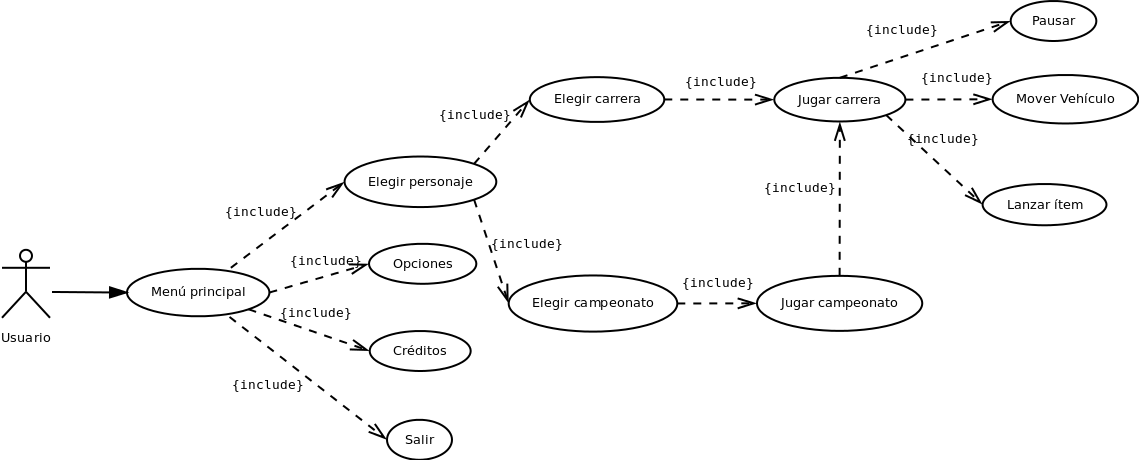
\includegraphics[scale=0.5]{imagenes/diagrama_casos.png}
  \end{center}
  \caption{Análisis: Diagrama de casos de uso}
\end{figure}

\subsection{Descripción de los casos de uso}

\paragraph{}
A continuación pasamos a la descripción de cada uno de los casoa de uso, para la cual usaremos una notación forma usando plantillas.
El texto debe ser legible y comprendido por un usuario que no sea experto.

\subsubsection{Caso de uso: Menú principal}

\begin{description}
    \item[Caso de uso] Menú principal
    \item[Descripción] Se muestra el menú principal de la aplicacion, donde es posible elegir uno de los modos de juego disponibles
    o acceder al menú de opciones.
    \item[Actores] Usuario
    \item[Precondiciones] Ninguna
    \item[Postcondiciones] Ninguna
    \item[Escenario principal] $\quad$
        \begin{enumerate}
            \item El sistema muestra el menú principal del juego en pantalla.
            \item El usuario selecciona la opción \textbf{carrera rápida}.
            \item El sistema inicia el modo de elección de personaje.
        \end{enumerate}
    \item[Extensiones --- flujo alternativo] $\quad$
        \begin{description}
            \item[*a ] El usuario cierra la ventana de la aplicación y sale de la aplicación
            \item[2a ] El usuario seleccion la opción \textbf{campeonato}.
            \begin{enumerate}
                \item El sistema inicia el modo de elección de personaje
            \end{enumerate}
            
            \item[2b ] El usuario seleccion la opción \textbf{contrarreloj}.
            \begin{enumerate}
                \item El sistema inicia el modo de elección de personaje
            \end{enumerate}
            
            \item[2c ] El usuario seleccion la opción \textbf{opciones}.
            \begin{enumerate}
                \item El sistema inicia las opciones
            \end{enumerate}
            
            \item[2d ] El usuario seleccion la opción \textbf{salir}.
            \begin{enumerate}
                \item El sistema sale de la aplicación.
            \end{enumerate}
            
        \end{description}
\end{description}

\subsubsection{Caso de uso: Elegir personaje}

\begin{description}
    \item[Caso de uso] Elegir personaje
    
    \item[Descripción] El usuario desea seleccionar el personaje con el que competirá en el juego, ya sea carrera rápida, 
    campeonato o contrarreloj.
    
    \item[Actores] Usuario
    
    \item[Precondiciones] El usuario ha elegido previamente en el menú principal una de las opciones: \textbf{carrera rápida},
    \textbf{campeonato} o \textbf{contrarreloj}
    
    \item[Postcondiciones] Se almacenará en la configuración de juego el jugador seleccionado para su posterior uso.
    
    \item[Escenario principal] $\quad$
        \begin{enumerate}
            \item El usuario debe seleccionar al jugador que usará en el juego.
            \item El sistema muestra el primer personaje junto a sus características.
            \item El usuario está satisfecho con su selección y pulsa el botón aceptar.
            \item El sistema almacena en la configuración el jugador seleccionado.
            \item El sistema pasa a selección de circuito, si la precondición es \textbf{carrera rápida} o \textbf{contrarreloj}
        \end{enumerate}
    \item[Extensiones --- flujo alternativo] $\quad$
        \begin{description}
            \item[*a ] El usuario cierra la ventana de la aplicación y sale de la aplicación
            
            \item[*b ] El usuario pulsa la opción cancelar.
            \begin{enumerate}
                \item El sistema vuelve al menú principal
            \end{enumerate}
            
            \item[3a ] El usuario no esta satisfecho con ese jugador y pulsa la flecha derecha.
            \begin{enumerate}
                \item El sistema muestra el siguiente jugador.
            \end{enumerate}

            \item[3b ] El usuario no esta satisfecho con ese jugador y pulsa la flecha izquierda.
            \begin{enumerate}
                \item El sistema muestra el anterior jugador.
            \end{enumerate}
            
        \end{description}
\end{description}

\subsubsection{Caso de uso: Elegir circuito}

\begin{description}
    \item[Caso de uso] Elegir circuito
    \item[Descripción] El usuario desea seleccionar el circuito en el que desea competir.
    \item[Actores] Usuario
    \item[Precondiciones] El usuario ha elegido previamente en el menú principal una de las opciones: \textbf{carrera rápida} 
    o \textbf{contrarreloj}
    \item[Postcondiciones] El sistema almacena en la configuración el circuito seleccionado.
    \item[Escenario principal] $\quad$
        \begin{enumerate}
            \item El usuario desea seleccionar el circuito en el que competir.
            \item El sistema muestra el primer circuito de todos los circuitos del campeonato actual.
            \item El usuario esta satisfecho con su elección, y pulsa el boton aceptar.
            \item El sistema almacena el circuito en la configuración del sistema.
            \item El sistema inicia la carrera.
        \end{enumerate}
    \item[Extensiones --- flujo alternativo] $\quad$
        \begin{description}
            \item[*a ] El usuario cierra la ventana de la aplicación y sale de la aplicación
            \item[*b ] El usuario pulsa la opcion cancelar.
            \begin{enumerate}
                \item El sistema vuelve a la selección de personaje.
            \end{enumerate}
            
            \item[3a ] El usuario no está satisfecho con ese circuito y pulsa sobre otro circuito del mismo campeonato.
            \begin{enumerate}
                \item El sistema muestra el nuevo circuito seleccionado.
            \end{enumerate}
            
            \item[3b ] El usuario no está satisfecho con los circuitos de ese campeonato y seleccionado otro campeonato.
            \begin{enumerate}
                \item El sistema muestra el primer circuito de los del campeonato seleccionado.
            \end{enumerate}
        \end{description}
\end{description}

\subsubsection{Caso de uso: Elegir campeonato}

\begin{description}
    \item[Caso de uso] Elegir campeonato
    \item[Descripción] El usuario desea seleccionar el campeonato que desea realizar.
    \item[Actores] Usuario
    \item[Precondiciones] El usuario ha elegido previamente en el menú principal una de las opciones: \textbf{campeonato}
    \item[Postcondiciones] El sistema almacena en la configuración todos lo circuitos del campeonato seleccionado.
    \item[Escenario principal] $\quad$
        \begin{enumerate}
            \item El usuario desea seleccionar el circuito en el que competir.
            \item El sistema muestra el primer circuito de todos los circuitos del campeonato actual.
            \item El usuario esta satisfecho con su elección, y pulsa el boton aceptar.
            \item El sistema almacena todos los circuitos del campeonato en la configuración del sistema.
            \item El sistema inicia la carrera.
        \end{enumerate}
    \item[Extensiones --- flujo alternativo] $\quad$
        \begin{description}
            \item[*a ] El usuario cierra la ventana de la aplicación y sale de la aplicación
            \item[*b ] El usuario pulsa la opcion cancelar.
            \begin{enumerate}
                \item El sistema vuelve a la selección de personaje.
            \end{enumerate}
            
            \item[3a ] El usuario pulsa sobre otro circuito del mismo campeonato.
            \begin{enumerate}
                \item El sistema muestra el nuevo circuito seleccionado.
            \end{enumerate}
            
            \item[3b ] El usuario no está satisfecho con los circuitos de ese campeonato y seleccionado otro campeonato.
            \begin{enumerate}
                \item El sistema muestra el primer circuito de los del campeonato seleccionado.
            \end{enumerate}
        \end{description}
\end{description}

\subsubsection{Caso de uso: Jugar carrera}

\begin{description}
    \item[Caso de uso] Jugar carrera
    \item[Descripción] El usuario juega una carrera
    \item[Actores] Usuario
    \item[Precondiciones] El usuario ha elegido previamente el personaje y el circuito donde jugar.
    \item[Postcondiciones] El usuario completa una carrera 
    \item[Escenario principal] $\quad$
        \begin{enumerate}
            \item El sistema carga el circuito.
            \item El sistema carga el jugador.
            \item El sistema carga la inteligencia artificial.
            \item El sistema muestra la pantalla de juego.
            \item El usuario y el sistema interactuan durante la carrera.
            \item El usuario completa la carrera.
            \item El sistema muestra las posiciones finales de la carrera.
            \item El usuario pulsa continuar.
            \item El sistema pasa a la siguiente pantalla dependiendo del modo de juego.
        \end{enumerate}
    \item[Extensiones --- flujo alternativo] $\quad$
        \begin{description}
            \item[*a ] El usuario cierra la ventana de la aplicación y sale de la aplicación
            
            \item[3a ] El sistema no carga la inteligencia artificial porque estamos en el modo campeonato.
            
            \item[8a ] El usuario pulsa reiniciar.
                \begin{enumerate}
                    \item El sistema renicia la carrea.
                    \item Volvemos al punto 1.
                \end{enumerate}
        \end{description}
\end{description}

\subsubsection{Caso de uso: Jugar campenato}

\begin{description}
    \item[Caso de uso] Jugar campeonato
    \item[Descripción] El usuario juega un campeonato.
    \item[Actores] Usuario
    \item[Precondiciones] El usuario selección previamente la opcion \textbf{campeonato} en el menú principal.
    \item[Postcondiciones] Se juega un campeonato.
    
    \item[Escenario principal] $\quad$
        \begin{enumerate}
            \item El usuario desea jugar un campenato
            \item El sistema carga el circuito actual
            \item El sistema y usuario interactuan en la carrera. Include Jugar carrera.
            \item Una vez terminada la carrera el sistema muestras las posiciones del campeonato.
            \item El usuario seleccion la opción continuar.
            \item El sistema pasar al siguiente circuito.
            \item Volvermos al punto 2.
        \end{enumerate}
    \item[Extensiones --- flujo alternativo] $\quad$
        \begin{description}
            \item[*a ] El usuario cierra la ventana de la aplicación y sale de la aplicación
            
            \item[2a ] Ya no hay más circuitos restantes.
                \begin{enumerate}
                    \item El sistema muestra la clasificación final de todos los jugadores del campeonato.
                    \item El usuario pulsa la opción continuar.
                    \item El sistema muestra la posición del jugador.
                \end{enumerate}
        \end{description}
\end{description}

\subsubsection{Caso de uso: Opciones}

\begin{description}
    \item[Caso de uso] Opciones
    \item[Descripción] El usuario desea modificar las opciones del juego.
    \item[Actores] Usuario
    
    \item[Precondiciones] El usuario seleccionó en el menú principal la opción \textbf{Opciones}.
    \item[Postcondiciones] El usuario modifica las opciones del juego.
    
    \item[Escenario principal] $\quad$
        \begin{enumerate}
            \item El usuario desea modificar las opciones del juego.
            \item El sistema muestra inicialmente las opciones de audio.
            \item El usuario modifica las distintas opciones de audio.
            \item El usuario esta conforme con los cambios realizados y pulsa sobre el botón aceptar.
            \item El sistema almacena todos los cambios en la configuración.
            \item El sistema vuelve al menú principal.
        \end{enumerate}
    \item[Extensiones --- flujo alternativo] $\quad$
        \begin{description}
            \item[*a ] El usuario cierra la ventana de la aplicación y sale de la aplicación.
            \item[*b ] El usuario selecciona la opción cancelar.
                \begin{enumerate}
                    \item El sistema vuelve al menú principal.
                \end{enumerate}
            
            \item [4a ] El usuario desea modificar las opciones de pantalla y pulsa sobre el boton de opciones de pantalla.
                \begin{enumerate}
                    \item El sistema muestra las opciones de pantalla.
                    \item El usuario modifica las distintas opciones de pantalla.
                \end{enumerate}
            
            \item [4b ] El usuario desea modificar las opciones de controles y pulsa sobre el boton de opciones de controles.
                \begin{enumerate}
                    \item El sistema muestra las opciones de controles.
                    \item El usuario modifica las distintas opciones de control.
                \end{enumerate}
            
        \end{description}
\end{description}

\subsubsection{Caso de uso: Salir}

\begin{description}
    \item[Caso de uso] Salir
    \item[Descripción] El usuario desea cerrar la aplicación.
    \item[Actores] Usuario
    \item[Precondiciones] Ninguna
    \item[Postcondiciones] Se sale de la aplicación.
    \item[Escenario principal] $\quad$
        \begin{enumerate}
            \item El usuario desea salir de la aplicación.
            \item El usuario pulsa la opción salir del menú principal.
            \item El sistema cierra la aplicación.
        \end{enumerate}
    \item[Extensiones --- flujo alternativo] $\quad$
        \begin{description}
            \item[*a ] El usuario cierra la ventana de la aplicación y sale de la aplicación
        \end{description}
\end{description}

%%%%%%%%%%%%%% MODELO CONCEPTUAL DE DATOS %%%%%%%%%%%%%%%%%%%5
\section{Modelo conceptual de datos}

\paragraph{}
Este apartado del análisis sirve para especificar los requisitos del sistema y las relaciones estáticas que
existen entre ellos.

\paragraph{}
Para este fin se utiliza como herramienta los diagramas de clase. En estos diagramas se representan
las clases de objetos, las asociaciones entre dichas clases, los atributos que componen las clases y las
relaciones de integridad.


\subsection{Diagrama de clases conceptuales}

\paragraph{}
En este apartado se muestra una lista con las diferentes clases necesarias para la realización de sistema. Junto a cada una de
las clases habrá una pequeña descripción sobre la labro que desempeña cada una.

\begin{description}
    \item [Juego] Clase principal de la aplicación, encargada de inicializar el sistema y el flujo entre unos apartados y otros.
    \item [Estado] Clase virtual, con las necesidades básicas de los estados del juego.
    
    \item [Menú Básico] Clase virtual, con las necesidades básicas de los menús.
    \item [Menú principal] Clase que gestiona el menú principal.
    \item [Menú selección personaje] Clase que gestiona el menú de selección de personaje.
    \item [Menú selección circuito] Clase que gestiona el menú de selección de circuito.
    \item [Menú opciones] Clase que gestiona el menú de opciones.
    \item [Cursor] Curso de los menús.
    \item [Boton] Clase que representa el botón en los menús.
    
    \item [Modo de juego] Clase virtual, con las necesidades básicas de los modos de juego.
    \item [Carrera rápida] Clase que gestiona el modo de juego carrera rápida.
    \item [Campeonato] Clase que gestiona el modo de juego campeonato.
    \item [Contrarreloj] Clase que gestiona el modo de juego contrarreloj.
    
    \item [Control de juego] Clase encargada del control de la carrera, controlando la interacción del jugador con el circuito, así 
    como el jugador con la inteligencia artificial. Aspectos básico como colisiones, scroll de pantalla, control de vueltas, control
    de posiciones.
    \item [Circuito] Clase encargada de cargar y dibujar el circuito.
    \item [Gestor de colisiones] Clase encargada de detectar y gestionar las colisiones.
    
    \item [Objeto de juego] Clase virtual con las necesidades básicas de los objetos del juego.
    \item [Caja de item] Clase que representa las cajas que proporcionan items a los jugadores.
    \item [Vehículo básico] Clase virtual con las necesidades básicas de los vehículos del juego.
    \item [IA] Clase que representa el comportamiento de los vehículos controlados por inteligencia artificial.
    \item [Jugador] Clase que que representa al vehículo controlado por el jugador.
\end{description}

\paragraph{}
En la siguiente imagen podemos ver el diagrama de clases asociado a los requisitos obtenidos:

\begin{figure}[H]
  \label{diagrama_clases_conceptuales}
  \begin{flushleft}
    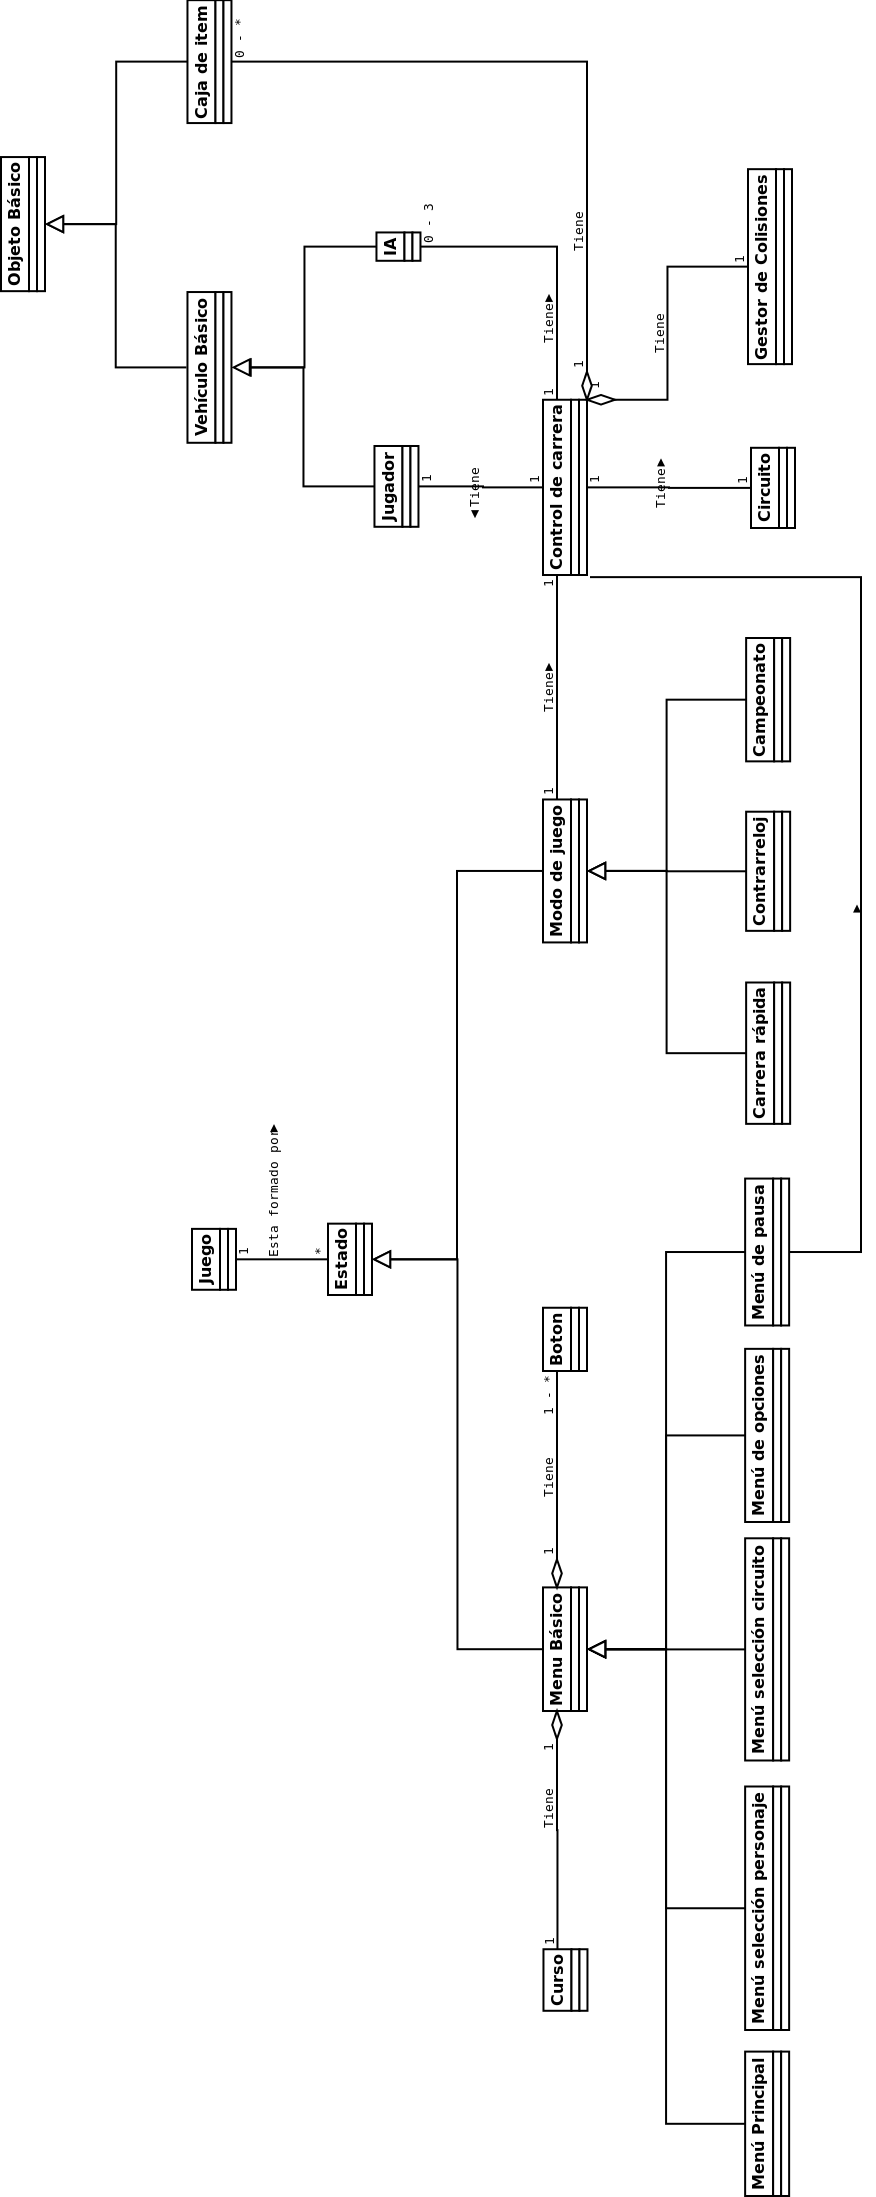
\includegraphics[scale=0.25]{imagenes/diagrama_clases_conceptuales.png}
  \end{flushleft}
  \caption{Análisis: Diagrama de clases conceptuales}
\end{figure}

\section{Modelo de comportamiento del sistema}

\paragraph{}
El modelo de comportamiento especifica como debe actuar el sistema. El sistema es el que engloba todos los objetos, y el modelo
consta de dos partes:

\begin{itemize}
    \item Diagramas de secuencias del sistema que muestra la secuencia de eventos entre el usuario y el sistema.
    \item Contrato de las operaciones del sistema, describen el efecto que producen las operaciones en el sistema.
\end{itemize}

\subsection{Diagramas de secuencias del sistema y contrato de las operaciones del sistema.}

\subsubsection{Modelo de comportamiento menú principal}

\textbf{Diagrama de secuencia}
\begin{figure}[H]
  \label{dia_menu_principal}
  \begin{center}
    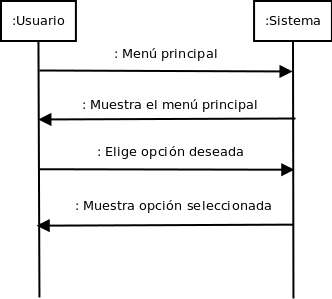
\includegraphics[scale=0.5]{imagenes/dia_menu_principal.png}
  \end{center}
  \caption{Análisis: Diagrama de secuencia Menú principal}
\end{figure}

\textbf{Contrato operaciones}

\begin{description}
    \item[Operación] Menú principal
    \item[Actores] Usuario, Sistema
    \item[Responsabilidades] Selecciona la opción principal del juego.
    \item[Precondiciones] Ninguna
    \item[Postcondiciones] Ninguna
\end{description}

\subsubsection{Modelo de comportamiento elegir personaje}

\textbf{Diagrama de secuencia}
\begin{figure}[H]
  \label{dia_elegir_jugador}
  \begin{center}
    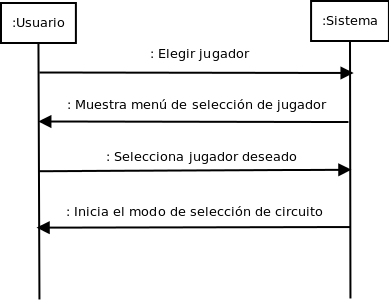
\includegraphics[scale=0.5]{imagenes/dia_elegir_jugador.png}
  \end{center}
  \caption{Análisis: Diagrama de secuencia Elegir jugador}
\end{figure}

\textbf{Contrato operaciones}

\begin{description}
    \item[Operación] Elegir personaje
    \item[Actores]  Usuario, sistema
    \item[Responsabilidades] Selecciona el personaje a controlar en el juego.
    \item[Precondiciones] Ha elegido previamente uno de los modos de juego en el menú principal.
    \item[Postcondiciones] Selecciona al personaje.
\end{description}

\subsubsection{Modelo de comportamiento elegir circuito}

\textbf{Diagrama de secuencia}
\begin{figure}[H]
  \label{dia_elegir_circuito}
  \begin{center}
    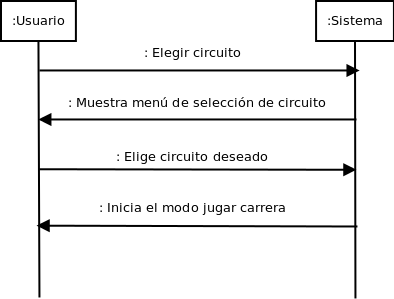
\includegraphics[scale=0.5]{imagenes/dia_elegir_circuito.png}
  \end{center}
  \caption{Análisis: Diagrama de secuencia Elegir circuito }
\end{figure}

\textbf{Contrato operaciones}

\begin{description}
    \item[Operación] Elegir circuito
    \item[Actores] Usuario, sistema
    \item[Responsabilidades] Selecciona el circuito donde competirá el jugador.
    \item[Precondiciones] Ha elegido previamente el personaje que competirá y el modo de juego carrera rápida o contrarreloj
    \item[Postcondiciones] Selecciona el circuito.
\end{description}

\subsubsection{Modelo de comportamiento elegir campeonato}

\textbf{Diagrama de secuencia}
\begin{figure}[H]
  \label{dia_elegir_campeonato}
  \begin{center}
    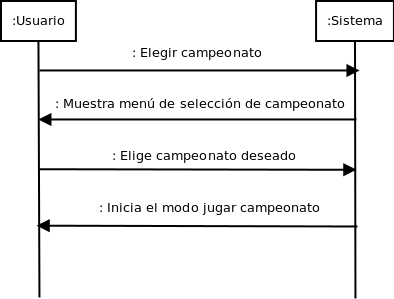
\includegraphics[scale=0.5]{imagenes/dia_elegir_campeonato.png}
  \end{center}
  \caption{Análisis: Diagrama de secuencia Elegir campeonato}
\end{figure}

\textbf{Contrato operaciones}

\begin{description}
    \item[Operación] Elige campeonato
    \item[Actores] Usuario, sistema
    \item[Responsabilidades] Seleccionar el campeonato en el que competirá el jugador.
    \item[Precondiciones] Ha elegido previamente el personaje que competirá y el modo de juego campeonato.
    \item[Postcondiciones] Selecciona el campeonato.
\end{description}

\subsubsection{Modelo de comportamiento jugar carrera}

\textbf{Diagrama de secuencia}
\begin{figure}[H]
  \label{dia_jugar}
  \begin{center}
    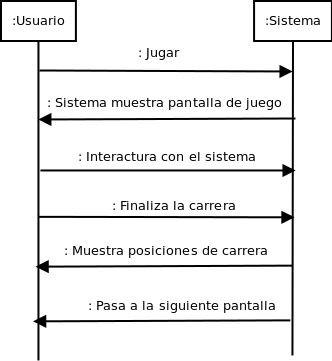
\includegraphics[scale=0.5]{imagenes/dia_jugar.png}
  \end{center}
  \caption{Análisis: Diagrama de secuencia Jugar carrera}
\end{figure}

\textbf{Contrato operaciones}

\begin{description}
    \item[Operación] Jugar
    \item[Actores] Usuario, sistema
    \item[Responsabilidades] Muestra la pantalla de juego desde la que el usuario puede jugar la partida.
    \item[Precondiciones] Previamente se han elegido jugador y circuito.
    \item[Postcondiciones] Un jugador gana la carrera.
\end{description}

\subsubsection{Modelo de comportamiento jugar campeonato}

\textbf{Diagrama de secuencia}
\begin{figure}[H]
  \label{dia_jugar_campeonato}
  \begin{center}
    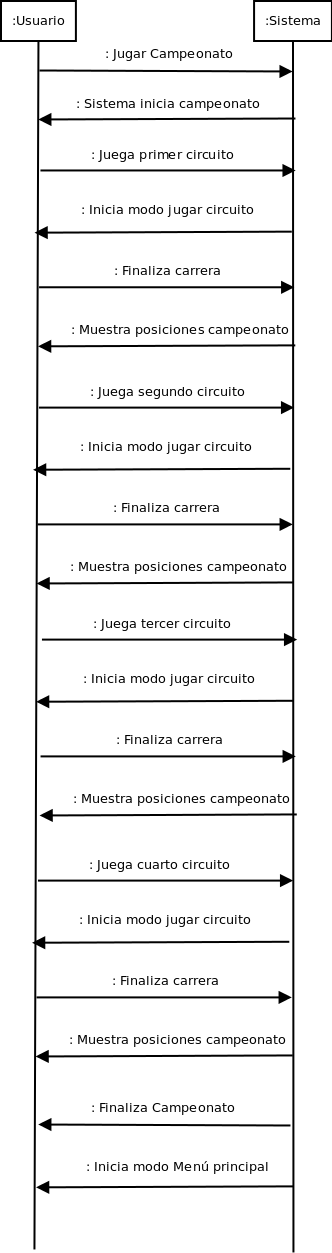
\includegraphics[scale=0.5]{imagenes/dia_jugar_campeonato.png}
  \end{center}
  \caption{Análisis: Diagrama de sencuancia Jugar campeonato}
\end{figure}

\textbf{Contrato operaciones}

\begin{description}
    \item[Operación] Jugar Campeonato
    \item[Actores] Usuario, sistema
    \item[Responsabilidades] Desarrolla todas la carreras del campeonato
    \item[Precondiciones] Se eligió el modo campeonato en el menú principal.
    \item[Postcondiciones] Un jugador gana el campeonato.
\end{description}

\subsubsection{Modelo de comportamiento opciones}

\textbf{Diagrama de secuencia}
\begin{figure}[H]
  \label{dia_opciones}
  \begin{center}
    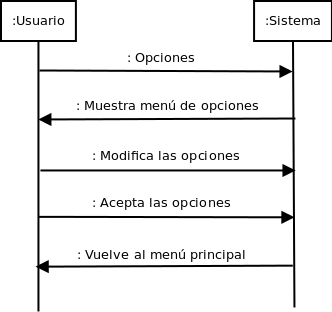
\includegraphics[scale=0.5]{imagenes/dia_opciones.png}
  \end{center}
  \caption{Análisis: Diagrama de secuencia opciones}
\end{figure}

\textbf{Contrato operaciones}

\begin{description}
    \item[Operación] Opciones
    \item[Actores] Usuairo, sistema
    \item[Responsabilidades] Se muestran las distintas opciones que el usuario puede modificar, como son el audio, pantalla y
    controles.
    \item[Precondiciones] Ninguna
    \item[Postcondiciones] Se modifican las opciones del juego.
\end{description}

\subsubsection{Modelo de comportamiento salir}

\textbf{Diagrama de secuencia}
\begin{figure}[H]
  \label{di_salir}
  \begin{center}
    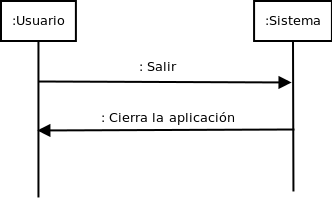
\includegraphics[scale=0.5]{imagenes/dia_salir.png}
  \end{center}
  \caption{Análisis: Diagrama de secuencia Salir}
\end{figure}

\textbf{Contrato operaciones}

\begin{description}
    \item[Operación] Salir
    \item[Actores] Usuario, Sistema
    \item[Responsabilidades] Permite al usuario salir del sistema
    \item[Precondiciones] Ninguna
    \item[Postcondiciones] Se sale de la aplicación
\end{description}

